\documentclass[../main.tex]{subfiles}
\graphicspath{
		{"../img/"}
		{"img/"}
}

\begin{document}
Na ostatnim wykładzie badaliśmy zbieżność szeregu postaci $a_k \psi_k$, gdzie $\psi_k$ - funkcje (wektory) własne operatora Sturma-Liouville'a spełniające dość dużą liczbę precyzyjnie zdefiniowanych warunków, dzięki którym operator S-L był samosprzężony i miał inne fajne własności (np. dodatnie wartości własne). Pamiętamy, że samosprzężoność operatora S-L wyznacza nam zbiór funkcji, którymi ten operator karmimy
\[
		\left( \left<f \left| Lg\right. \right> = \left<Lf \left| g\right. \right>  \right)
.\]
Czyli zbiór funkcji całkowalnych z kwadratem na jakiejś dziedzinie.
\begin{przyklad}
		$L = -\frac{d^2}{dx^2}$, na zbiorze $U = \left\{ u\in \mathcal{L}^2([0,1]), u(0) = u(1) = 0 \right\} $. Do zbioru $U$ należą wektory własne operatora $L$, czyli
		\[
		\psi_n = \sin n\pi x,\quad \lambda_n = n^2\pi^2
		.\]
		Jak i funkcji, które mogłyby być warunkami początkowymi, gdybyśmy chcieli rozwiązać równanie różniczkowe. Na przykład do $U$ należy funkcja $u_1 = x(1-x)$.
\end{przyklad}
Na ostatnim wykładzie pokaaliśmy, że baza $\psi_n$ jest zupełna, tzn. każdą funkcję $f$ należącą do zbioru funkcji klasy $\mathcal{L}^2$, na którym operator $S-L$ jest samosprzężony da się przedstawić jako granicę ciągu $a_k\psi_k$, gdzie $a_k = \left<f \left| \psi_k\right. \right> $ i zbieżność ta jest w $\mathcal{L}^2$ jednostajna.
Czyli na przykład
\[
		x(1-x) = a_k \sin k\pi x
.\]
\textbf{Dygresja:} swoją drogą możemy policzyć $R(u_1)$, gdzie $R$ jest operatorem Reynoldsa
\[
		R(u) = \frac{\left<Lu \left| u\right. \right> }{\left<u \left| u\right. \right> }
.\]
W naszym przypadku: $Lu_1 = -\frac{d^2}{dx^2}\left( x\left( 1-x \right)  \right) = 2.$
\[
		\left<2 \left| x(1-x)\right. \right> = \int\limits_0^1 2\cdot x(1-x)dx = \frac{1}{3}
.\]
\[
		\left<u_1 \left| u_1\right. \right> = \int\limits_0^1 x(1-x)x(1-x)dx = \frac{1}{30}
.\]
Zatem
\[
		R(u_1) = \frac{1}{3} / \frac{1}{30} = 10
.\]
I co z tego? A to, że pamiętamy, o tym, że $R(u)$ osiąga minimum na wektorach własnych i to minimumjest najmniejszą wartością własną, czyli
\[
		R(u) \ge \lambda_1 \underset{u\in U}{\forall} \implies 10\ge 1^2 \pi^2
.\]
No, zgadza się.\\
Pamiętamy, że zbieżność jednostajna w $\mathcal{L}^2$ nie oznacza zbieżności w $\mathcal{L}^1$ i szereg fouriera jest w $\mathcal{L}^1$ zbieżny punktowo. Może być zbieżny jednostajnie, gdy na $\mathcal{L}^1$ nałożymy dodatkowe warunki.
\begin{pytanie}
		Jak otrzymane twierdzenia mają się do równań cząstkowych i metody separacji zmiennych?
\end{pytanie}
\textbf{Odpowiedź:} Zależy o co pytamy i od takich pojęć jak \textit{problem dobrze postawiony}.
\begin{definicja}
		Problem jest dobrze postawiony, jeżeli o równaniu różniczkowym możemy powiedzieć, że
		\begin{itemize}
				\item rozwiązania istnieją
				\item są jednoznaczne
				\item są ciągłe ze względu na zmianę warunków początkowych.
		\end{itemize}
\end{definicja}
Zupełność układu funkcji własnych operatora S-L związana jest z istnieniem i jednoznacznością oraz z teorią funkcji specjalnych. Ogólnej teorii dla dowolnego równania różniczkowego nie ma. Mamy trochę wyników dla konkretnych równań fizyki matematycznej, które sprowadzają się do nałożenia warunków dodatkowych na funkcje z $\mathcal{L}^2$, co gorsza, niedziała warunek na "niefizyczność" (przykłady niedługo). Na szczęście, możemy też od czasu do czasu powiedzieć coś konstruktywnego - przykład takiej analizy przeprowadzimy dla równania falowego.
\subsection{Równanie falowe - motywacja}
Jak dojść do równania falowego? najprościej tak:\\
Niech
\[
A = -\phi dt + A_x dx + A_ydy + A_zdz
,\]
jednoforma potencjału elektromagnetycznego. Wówczas $F = dA$ i $dF = 0$ - mamy trzy równania falowe i jedno równanie Laplace'a.\\
Wariant trudniejszy - wyobraźmy sobie funkcję, której wartość zależy od średniej wartości funkcji w otoczeniu. Możemy ten warunek zapisać jako
\[
		\varphi(x) = \frac{\varphi(x+h) - \varphi(x-h)}{2}
,\]
$h$ - odpowiednio małe, $\varphi: U\subset\mathbb{R}^n\to \mathbb{R}$. Moglibyśmy teraz pomyśleć o funkcji $\varphi(x,t)$, której dynamika (przyspieszenie) zależy od średniej wartości zmian w okolicy, czyli
\[
		"ma" = \varphi(x,t)_{,t t} = \frac{\varphi(x+h) - \varphi(x-h)}{2} - \varphi(x)
.\]
Ale
\begin{align*}
		& \frac{1}{2}\left[ \varphi(x+h) + \varphi(x-h) - 2\varphi(x) \right] = \\
		&= \frac{1}{2}\left[ \varphi(y+2h) + \varphi(y) - \varphi(y+h) - \varphi(y+h) \right] = \\
		&= \frac{1}{2}\left[ \varphi((y+h)+h) - \varphi(y+h) - \left( \varphi(y+h) - \varphi(y) \right)  \right] = \\
		&= \frac{1}{2}\left[ \varphi'(y+h) h + r_1(y+h) - \left( \varphi'(y)h + r_2(y) \right)  \right] = \\
		&= \frac{1}{2}\left[ h \left( \varphi'(y+h) - \varphi'(y) \right) + r_1(y+h) - r_2(y) \right] = \\
		&= \frac{1}{2}\left[ \varphi''(y)hh + r_3(y+h)h + r_1(y+h) - r_2(y) \right]
.\end{align*}
Czyli jeżeli zachodanie funkcji zależy od średniego odchylenia, to
$\varphi_{,t t}\sim \varphi''$ (bo druga pochodna po czasie też jest rzędu $h^2$). Dla przypadku statycznego wychodzi $\varphi'' = 0$ i ogólniej $\Delta \varphi = 0$.
\begin{przyklad}
		Dla ruchu jednowymiarowego
		\[
		\begin{cases}
				u_{,t t} = c^2 u_{,x x} & \\
				u(x,0) = f(x) & x\in R, t>0\\
				u_{,t}(x,0)  = g(x)
		\end{cases}
		.\]
\end{przyklad}
\begin{pytanie}
		Jak wyprowadzić równanie falowe z równania ciągłości?
\end{pytanie}
Problem typu $u_{,tt}(x,t) = c^2 u_{,x x}$ rozważaliśmy już w drugim semestrze przy okazji zamiany zmiennych
\begin{align*}
		x = \xi + \eta\\
t = \xi - \eta
.\end{align*}
Dzięki której równanie zmieniło się na dużo fajniejszą formę
\[
\frac{\partial ^2 u}{\partial \xi \partial \eta } = 0
.\]
W efekcie dostaliśmy
\[
		u(x,t) = \alpha(x-ct) + \beta(x+ct)
.\]
Zatem
\begin{align*}
		f(x) &= \alpha(x) + \beta(x)\\
		g(x) &= -c\alpha'(x) + c\beta(x)
.\end{align*}
No i tam ostatecznie wyszło
\[
		u(x,t) = \frac{f(x-ct) + f(x+ct)}{2} + \frac{1}{c} \int\limits_{x-ct}^{x+ct} g(s)  d s
,\]
gdzie $f\in \mathcal{C}^2$ i $g\in \mathcal{C}^1$. Warunki na $f$ i $g$ można osłabić przepisując równanie falowe w postaci całkowej dla słabych rozwiązań
\[
		\int\limits_0^\infty dt \int\limits_\mathbb{R} dx \left[ u_{,t t} - c^2 u_{,x x} \right] v(t,x) = 0 \underset{v(t,x)\in \text{funkcje próbne}}{\forall}
.\]
Zauważmy, że w przeciwieństwie do równania przewodnictwa w rozwiązaniach równania falowego pojawia się wreszcie wpływ skończonej prędkości przekazywania informacji.
\begin{pytanie}
		Jak przełożyć na język $f(x)$ i $g(x)$ szarpnięcie struny nieskończonej?
		Jeżeli na przykład $f$ - trójkąt i $g(x) \equiv 0$, to jak będzie zachowywał się taki impuls?
		\begin{figure}[h]
				\centering
				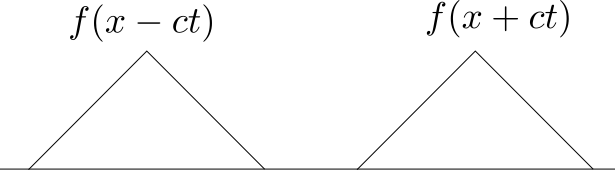
\includegraphics[width=0.6\textwidth]{zabki}
				\caption{Zachowanie impulsu}
				\label{fig:zabki}
		\end{figure}
\end{pytanie}
Nie rozmyje się, więc klaśnięcie w 1-D usłyszymy precyzyjnie, niezależnie od tego jak daleko będziemy, tylko trzeba chwilę poczekać. Co będzie gdy klaśniemy w 2-D? W 3-D jest ważniejsze, ale sprawdzimy czy na przykład 2-D zachowuje się tak samo. W fizyce materiałów, tam gdzie występują przerwy energetyczne na przykład 2-D działa. Rzeczywistość może być czasami opisywana przez 2-D.
\begin{przyklad}
		Struna półnieskończona\\
		Mając rozwiązania dla struny nieskończonej
		\begin{equation}
				\label{eq:wave-ex}
				u(x,t) = \frac{f(x+ct) + f(x-ct)}{2} + \frac{1}{2c} \int\limits_{x-ct}^{x+ct}g(s)d s
		\end{equation}
		chcemy znaleźć rozwiązania problemu
\[
\begin{cases}
		u_{,t t} = c^2 u_{x x}&t>0,x>0\\
		u(x,0) = f(x) & x\ge 0\\
		u_{,t}(x,0) = g(x) & x\ge 0\\
		u(0,t) = 0& t \ge 0
\end{cases}
.\]
Widzimy, że gdy $x\ge ct$, to rozwiązania będą takie jak wcześniej - nie zauważymy nawet, że warunki brzegowe nie są określone dla $(x<0,t=0)$. Wróćmy do wyprowadzenia wzoru typu \ref{eq:wave-ex}. Wiemy, że
\[
		u(x,t) = \alpha(x-ct) + \beta(x+ct)
,\]
ale dla $x-ct < 0$ nie mamy informacji o $\alpha(x-ct)$. Za to wiemy, że $u(0,t\ge0) = 0$, czyli
\begin{align*}
		0 &= \alpha(-ct) + \beta(ct),\quad t>0\\
		0 &= \alpha(-s) + \beta(s),\quad t>0,u(x,0) = f(x),x>0\\
		f(x) &= \alpha(x) + \beta(x),\quad x>0
.\end{align*}
		Zatem $\alpha(-s) = -\beta(s)$, $s>0$ i wiemy, czym zastąpić $\alpha$ na ujemnych wartościach.\\
		$\beta(x)$ liczymy dla $x>0 $ tak jak poprzednio
		\[
				\beta(x) = \frac{1}{2}f(x) + \frac{1}{2c}\int\limits_{x_0}^{x}g(s)d s,\quad x > 0
		.\]
		Ale gdy $x - ct \le 0$, to $ct - x \ge 0$ i wtedy
		\[
				u(x,t) = \frac{f(x+ct) - f(ct-x)}{2} + \frac{1}{2c}\int\limits_{ct-x}^{ct+x}g(s)d s
		.\]
		Możemy to zapisać jako
		\begin{align*}
				u(x,t) = \begin{cases}
						\frac{\partial }{\partial t} \frac{1}{2c}\int\limits_{ct-x}^{ct+x}f(s) d s + \frac{1}{2c}\int\limits_{ct-x}^{ct+x}g(s)d s,&x - ct < 0\\
						\frac{f(x-ct) + f(x+ct)}{2} + \frac{1}{2c}\int\limits_{x-ct}^{x+ct}g(s) d s & x-ct > 0
\end{cases}
		.\end{align*}
\end{przyklad}
\end{document}

